\section{Exercise one}

Given the system: 
\[\begin{cases}
    x(t+1)=3x(t)+2v(t) \\
    y(t)=2x(t)-v(t)
\end{cases} \qquad v(t) \sim WN(0,1)\]
Assuming $v(t)$ is the initial position $x(1)$, we are asked to:
\begin{enumerate}
    \item Compute the time variant one-step ahead Kalman predictor.
    \item Compute the asymptotic Kalman gain of the one-step ahead predictor using the graphical method.
    \item Check the existence of the Kalman predictor using asymptotic Kalman filter theorems.
    \item Compute the transfer function from $y(t)$ to $\hat{y}(t+1|t)$. 
    \item Compute the variance of $e_y(t)=y(t)-\hat{y}(t|t-1)$. 
    \item Find the state equation of the Kalman filter $\hat{x}(t|t)$. 
\end{enumerate}

\subsection*{Solution}
\begin{enumerate}
    \item We define two White Noises as $v_1(t)=2v(t)$, and $v_2(t)=-v(t)$: 
        \[V_1=\text{Var}\left[v_1(t)\right]=\mathbb{E}\left[v_1(t)v_1(t)^T\right]=4\mathbb{E}\left[v(t)v(t)^T\right]=4\]
        \[V_2=\text{Var}\left[v_2(t)\right]=\mathbb{E}\left[v_2(t)v_2(t)^T\right]=(-1)^2\mathbb{E}\left[v(t)v(t)^T\right]=1\]
        \[V_{12}=\mathbb{E}\left[v_1(t)v_2(t)^T\right]=-2\mathbb{E}\left[v(t)v(t)^T\right]=-2\]
        We can now write the Differential Riccati Equation for scalar problems:
        \begin{align*}
            P(t+1)  &=F^2P(t)+V_1-(FHP(t)+V_{12})(H^2P(t)+V_2)^{-1}(FHP(t)+V_{12}) \\
                    &=F^2P(t)+V_1-\dfrac{(FHP(t)+V_{12})^2}{(H^2P(t)+V_2)^{-1}} \\
                    &=\dfrac{F^2H^2P^2(t)+(H^2V_1+F^2V_2)P(t)+V_1V_2-F^2H^2P^2(t)-V_{12}^2-2FHV_{12}P(t)}{(H^2P(t)+V_2)^{-1}} \\
                    &=\dfrac{(H^2V_1+F^2V_2)P(t)+V_1V_2-V_{12}^2-2FHV_{12}P(t)}{(H^2P(t)+V_2)^{-1}} \\
                    &=\dfrac{49P(t)}{4P(t)+1} \\
        \end{align*}
        The Kalman gain is computed as:
        \[k(t)=\left(FHP(t)+V_{12}\right)\left(H^2P(t)+V_2\right)^{-1}=\dfrac{6P(t)-2}{4P(t)+1}\]
        So the predictor becomes:
        \[\begin{cases}
            \hat{x}(t+1|t)=3\hat{x}(t|t-1)+k(t)\left(y(t)-\hat{y}(t|t-1)\right) \\ 
            \hat{y}(t|t-1)=2\hat{x}(t|t-1) \\
            k(t)=\dfrac{6P(t)-2}{4P(t)+1} \\
            P(t+1)=\dfrac{49P(t)}{4P(t)+1}
        \end{cases}\]
        The state equation can be rewritten as:
        \[\hat{x}(t+1|t)=(3-2k(t))\hat{x}(t|t-1)+k(t)y(t)\]
    \item We compute the solutions of the Algebraic Riccati Equation
        \[\bar{P}=\dfrac{49\bar{P}}{4\bar{P}+1}\rightarrow\bar{P}_{1,2}=0,12\]
        Both solutions are greater than or equal to zero, making them acceptable. 
        The graph of $P(t+1)$ is shown below:
        \begin{figure}[H]
            \centering
            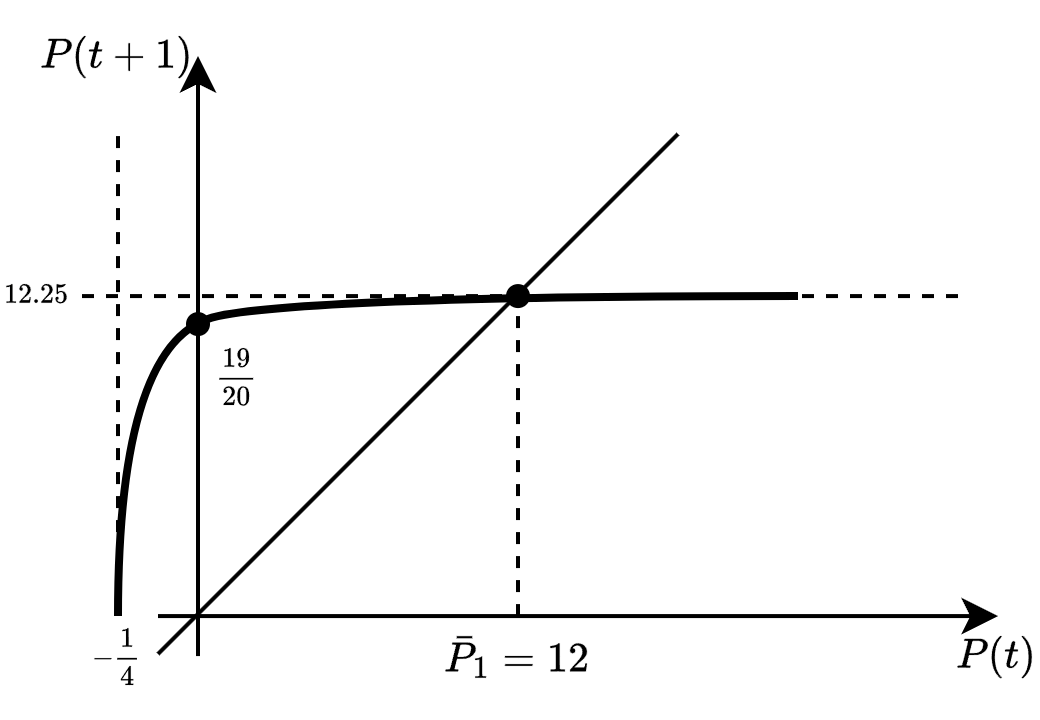
\includegraphics[width=0.5\linewidth]{images/ex.png}
        \end{figure}
        Next, we check the convergence in three cases:
        \begin{itemize}
            \item $P_0=0$: converges to $P=0$. 
                In this case, the Kalman static gain is $\bar{K}=-2$. 
                With this gain, $F-\bar{K}H=7>1$, indicating that the system is unstable.
            \item $P_0>0\:\land\:P_0\leq\bar{P}$: converges to $\bar{P}=12$.
                The Kalman static gain in this case is  $\bar{K}=\frac{10}{7}$. 
                With this gain, $F-\bar{K}H=\frac{1}{7}<1$, showing that the system is asymptotically stable.
            \item $P_0>\bar{P}$: converges to $\bar{P}=12$. 
                The stability is the same as in the previous case.
        \end{itemize}
        In conclusion, for the system to be asymptotically stable, $P_0$ must be greater than zero.
    \item One requirement for both theorems is that $V_{12}=0$. 
        In our case, $V_{12}\neq 0$, so we cannot apply the theorems.
    \item The predictor is (with the gain found before):
        \[\begin{cases}
            \hat{x}(t+1|t)=3\hat{x}(t|t-1)+\dfrac{10}{7}y(t)-\dfrac{10}{7}\hat{y}(t|t-1) \\
            \hat{y}(t|t-1)=2\hat{x}(t|t-1)
        \end{cases}\]
        By substituting the second equation into the first one, we obtain:
        \[\begin{cases}
            \hat{x}(t+1|t)=\dfrac{1}{7}\hat{x}(t|t-1)+\dfrac{10}{7}y(t) \\
            \hat{y}(t|t-1)=2\hat{x}(t|t-1)
        \end{cases}\]
        The transfer function from $y(t)$ to $\hat{y}(t|t-1)$ is computed as: 
        \[W(z)=\tilde{H}(zI-\tilde{F})^{-1}\tilde{G}=\dfrac{\frac{20}{7}}{z-\frac{1}{7}}\]
        But since we need the transfer function from $y(t)$ to $\hat{y}(t+1|t)$ we multiply by $z$, yielding: 
        \[W(z)=\dfrac{\frac{20}{7}z}{z-\frac{1}{7}}\]
    \item We have that: 
        \begin{align*}
            \text{Var}[e_y(t)]  &=\text{Var}\left[y(t)-\hat{t}(t|t-1)\right] \\
                                &=\text{Var}\left[H\left((x|t)-\hat{x}(t|t-1)\right)+v_2(t)\right]
        \end{align*}
        Since the White Noise $v_2(t)$ only affects $y(t)$, it remains independent from the state $x(t)$.
        At time $t$, $\hat{x}(t|t-1)$ is influenced by all White Noise $v_2(t-\tau)$ with $\tau \geq 1$, thereby being independent from $v_2(t)$. 
        Considering these factors, we derive:
        \begin{align*}
            \text{Var}[e_y(t)]  &=\text{Var}\left[H\left((x|t)-\hat{x}(t|t-1)\right)+v_2(t)\right] \\ 
                                &=\text{Var}\left[H\left((x|t)-\hat{x}(t|t-1)\right)\right]+\text{Var}\left[v_2(t)\right] \\
                                &=\text{Var}\left[He_x(t)\right]+V_2 \\
                                &HP(t)H^{T}+V_2 =4P(t)+1
        \end{align*}
        In the asymptotic scenario where $P(t)\rightarrow 12$, we obtain:
        \[\text{Var}[e_y(t)]=48+1\]
    \item Based on the provided information:
        \[F=3 \quad G=0 \quad H=2 \quad V_1=4 \quad V_2=1 \quad V_{12}=-2\]
        and also:
        \[\bar{P}=12 \quad \bar{K}=\dfrac{10}{7} \quad F-\bar{K}H=\dfrac{1}{7}\]
        Since the matrix $F$ is invertible, we can deduce:
        \[\hat{x}(t|t)=\dfrac{1}{3}\hat{x}(t+1|t)=\dfrac{1}{21}\hat{x}(t|t-1)+\dfrac{10}{21}y(t)\]
        Recalling that $3\hat{x}(t-1|t-1)=\hat{x}(t|t-1)$, we derive: 
        \[\hat{x}(t|t)=\dfrac{1}{7}\hat{x}(t-1|t-1)+\dfrac{10}{21}y(t)\]
\end{enumerate}